\subsection{External interfaces requirements}
\begin{enumerate}[label=\textbf{R\arabic*}]
    \item The \ac{eMSP} must allow the users to register (providing email, password, payment method and his infos);
    \item The \ac{CPMS} must allow the \acp{CPO} to register (providing email, password, id-station, partita iva, number of possible charging slots);
    \item The system must allow the \acp{CPO} to modify the possible charging slots in their stations;
          % Maybe not useful anymore R4
    \item The system must verify the correctness of the identification data for the \acp{CPO};
    \item The system must allow the user to login;
    \item The system must allow the user to choose a specific station, a timeslot;
    \item The system must notify the user when the charging process is finished via a notification;
    \item The \ac{CPMS} must allow the \acp{CPO} to choose the mode (manual or automatic) of operation
\end{enumerate}

\subsubsection{User interfaces}
\paragraph{\ac{eMSP}}
The \ac{eMSP} should be accessible to the user through an application installed on the mobile device.
The first interface shown to the user is the \textit{login} page where the user have to input the username (or e-Mail) and password in order to authenticate.
From the \textit{login} page there is also the the possibility to go to the \textit{register} page where the fields for inputting the necessary informations are present.
After logging in, there are multiple views available to the user, corresponding of multiple tabs in the app, which are: 
\begin{itemize}
    \item A map of the charging stations near the position of the user;
    \item A ranked list personalizable in base of parameters chosen by the user (nearer, cheaper, more environment friendly\ldots).
    \item A screen for enabling/disabling suggestions from the system, setting up the connection to the user online calendar and, when the connection is present, it also shows a view of the appointments on the calendar.
\end{itemize} 
Clicking on one station (from the ranked list or the map) the specific informations about the station are shown, along with a calendar (and if the system is synchronized with the user calendar, it shows also the days with some appointment scheduled). Once selected the wanted date, a timeline of  the day is shown, with in green the available times and in red the moments when the station is full.

\paragraph{\ac{CPMS}}


\subsubsection{Hardware interfaces}
\subsubsection{Software interfaces}
\subsubsection{Communication interfaces}

\subsection{Functional requirements}

\begin{enumerate}[label=\textbf{R\arabic*}]
    \item The system must provide information () about the stations nearby;
    \item The system must reserve a position for a user who registered for a charge through the application;
    \item The system mustn't have collisions in the booking of charges; (non si possono registrare più di X user per timeslot sovrapposti)
    \item The system must take the service money from the user payment method after the charging is finished;
\end{enumerate}
\clearpage
\subsubsection{Use case diagrams}
\begin{figure}[!h]
    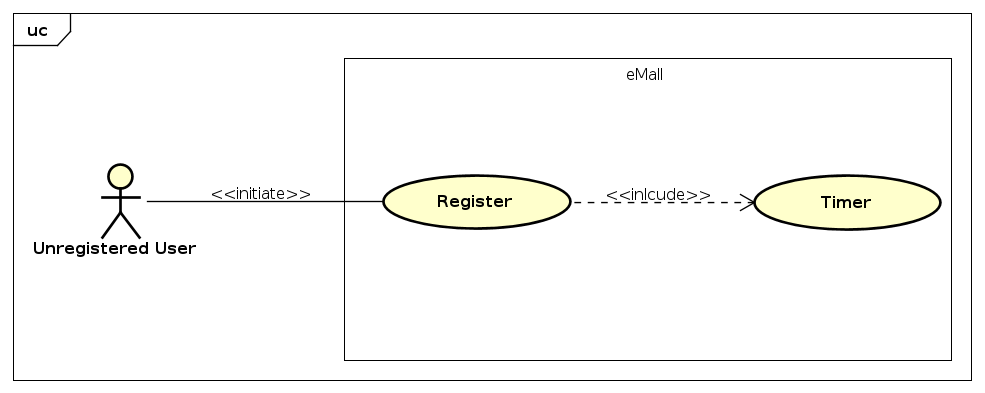
\includegraphics[keepaspectratio, width=16cm]{UseCase/UnregisteredUser.png}
    \caption{Unregistered user use case}
\end{figure}
\begin{figure}[!h]
    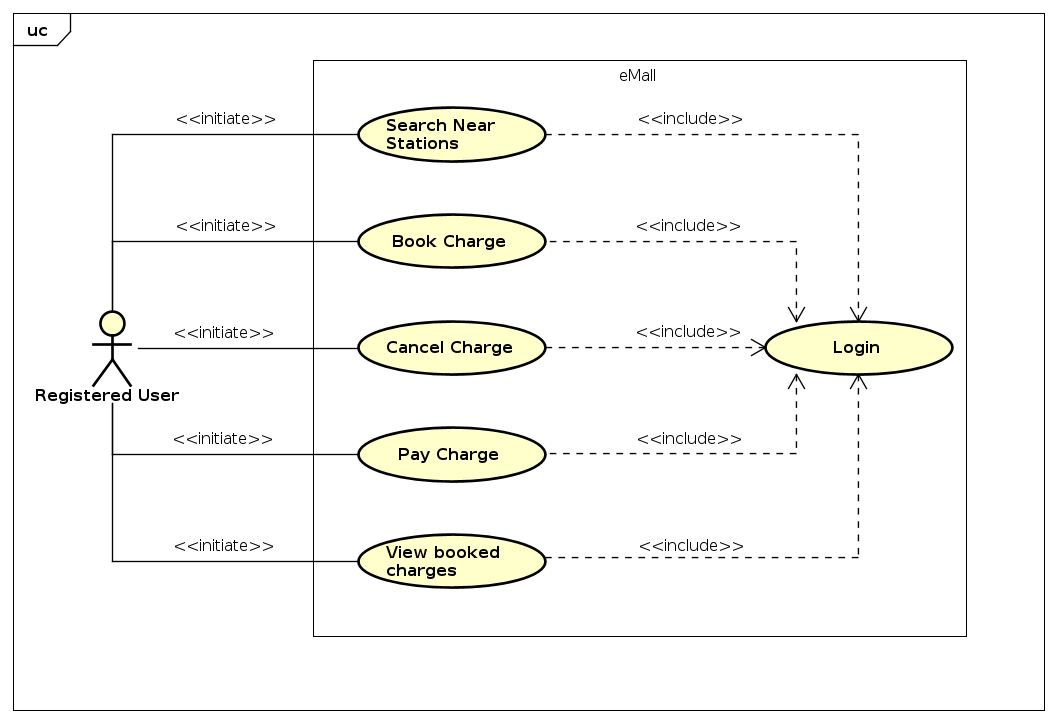
\includegraphics[keepaspectratio, width=16cm]{UseCase/RegisteredUser.png}
    \caption{Registered user use case}
\end{figure}
\subsubsection{Sequence diagrams}
\todo[inline]{Per quanto riguarda il sistema CPMS, come si "registra" il CPO maintainer?\\Nell'UML forse conviene chiamare l'interfaccia eMSP e poi l'attore che la implementa eMall. In questo modo possiamo far sì che le charging sockets utilizzino quell'interfaccia per poter ricavare le info sulla carica quando un utente inserisce il codice.}
Below there are some sequence diagrams to show how the basic actions should be over time.
\todo[inline]{Correggere sequence perform a charge, c'è un sync message tra chargingSocket ed eMall "updateChargingStatus" che non restituisce controllo}
\begin{figure}[!h]
    \begin{center}
        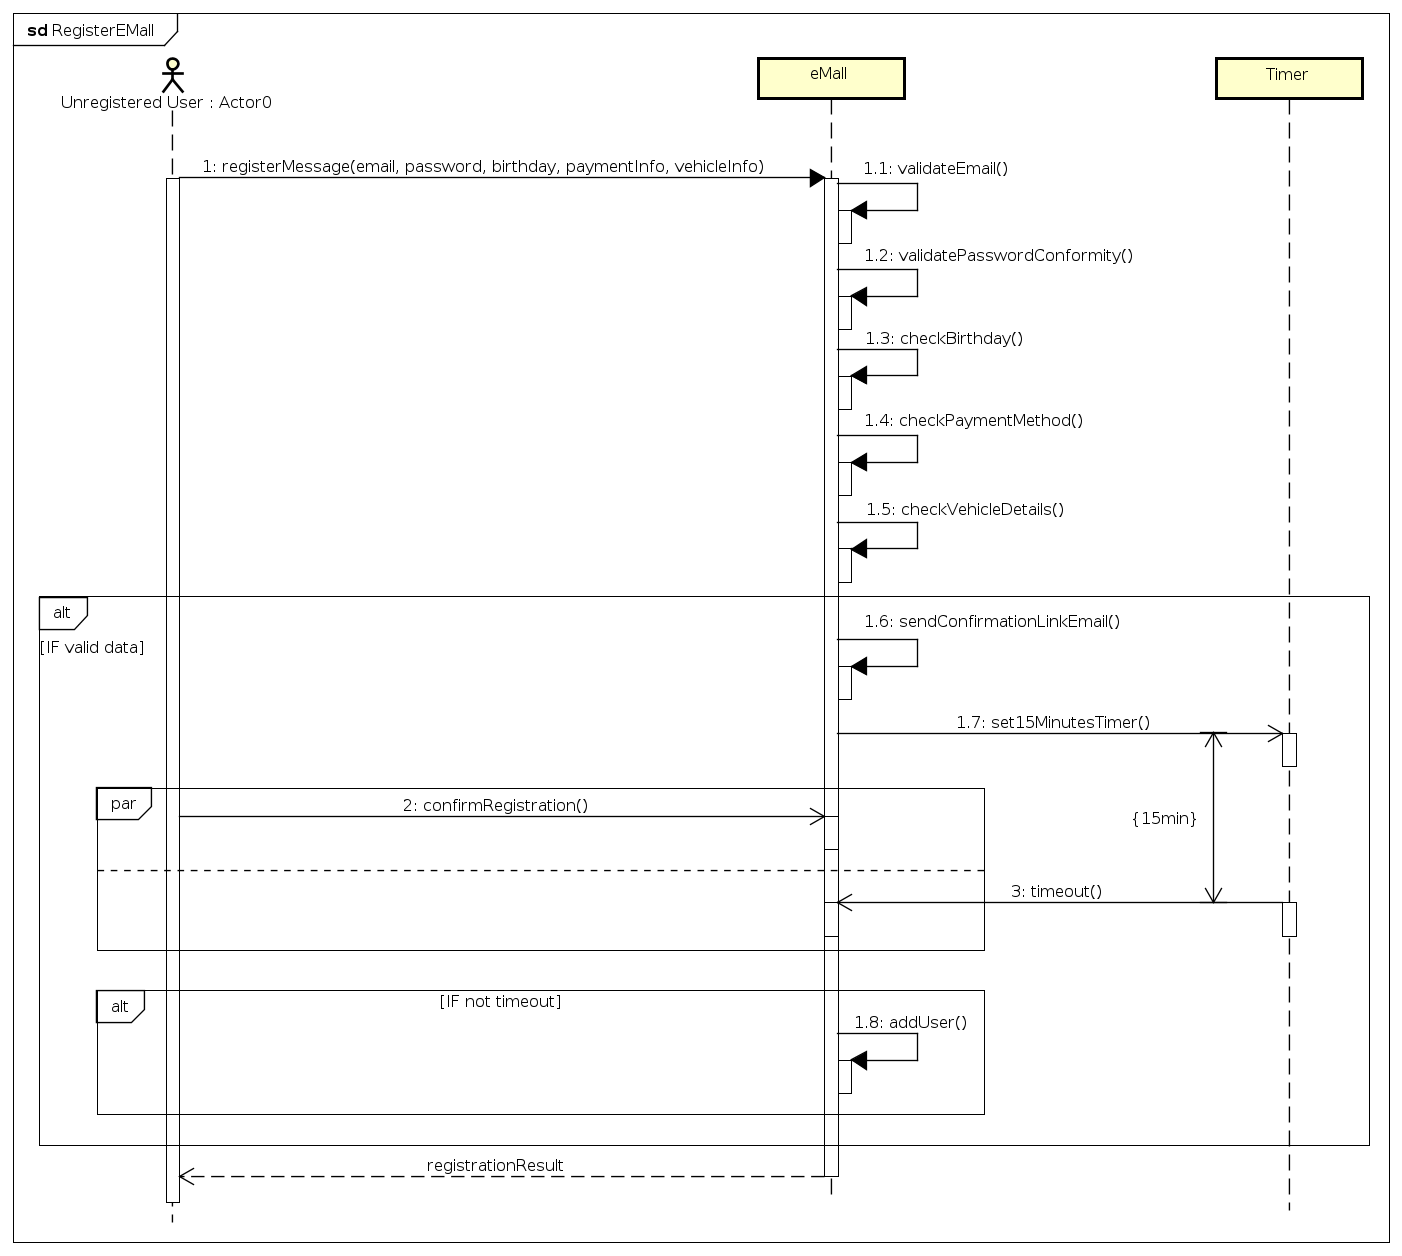
\includegraphics[keepaspectratio, width=16cm]{Sequence/RegisterEMall.png}
        \caption{Registration into \ac{eMall} sequence}
    \end{center}
\end{figure}
\begin{figure}[!h]
    \begin{center}
        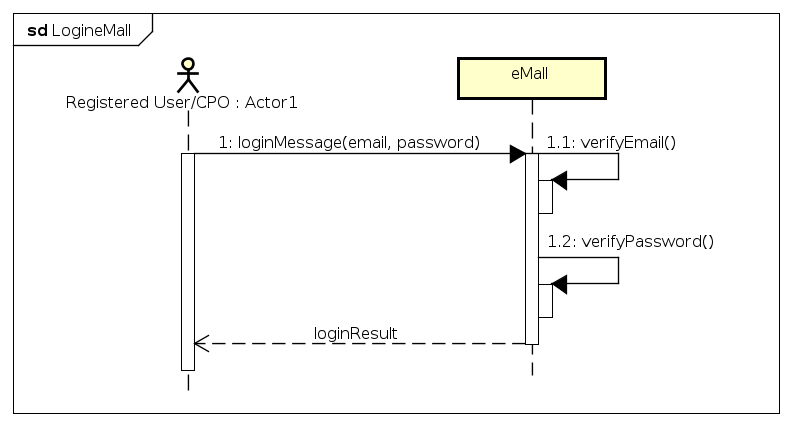
\includegraphics[keepaspectratio, width=16cm]{Sequence/LoginEMall.png}
        \caption{Login into \ac{eMall} sequence}
    \end{center}
\end{figure}
\begin{figure}[!h]
    \begin{center}
        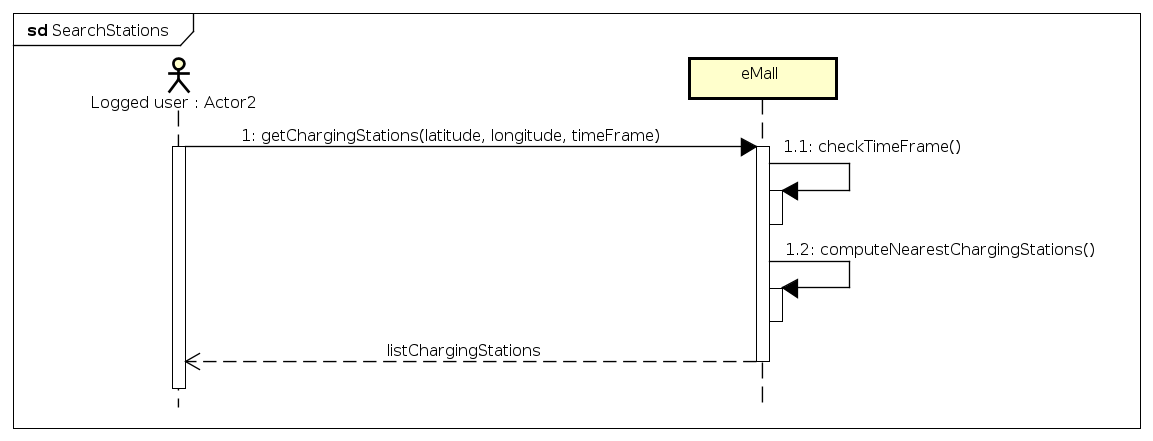
\includegraphics[keepaspectratio, width=16cm]{Sequence/SearchStations.png}
        \caption{Get the nearby charging stations}
    \end{center}
\end{figure}
\begin{figure}[!h]
    \begin{center}
        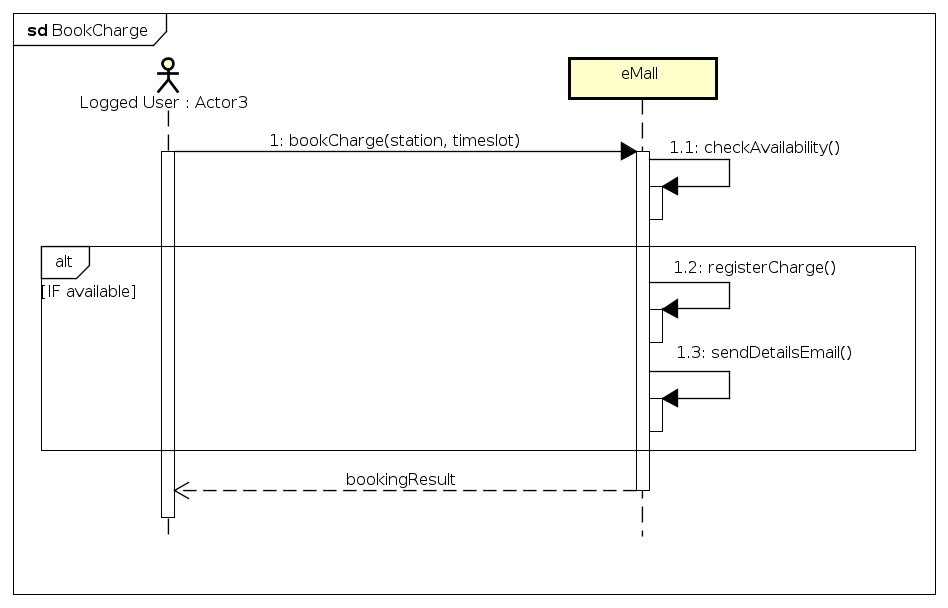
\includegraphics[keepaspectratio, width=16cm]{Sequence/BookCharge.png}
        \caption{Book a charge sequence}
    \end{center}
\end{figure}
\begin{figure}[!h]
    \begin{center}
        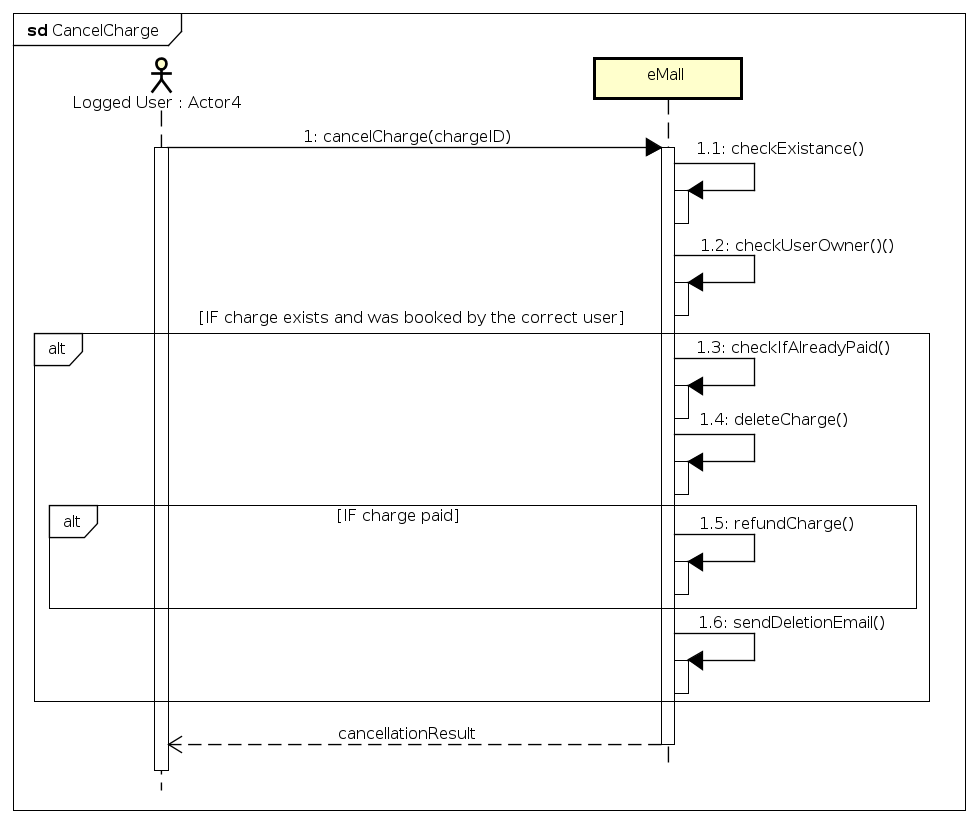
\includegraphics[keepaspectratio, width=16cm]{Sequence/CancelCharge.png}
        \caption{Cancel a charge sequence}
    \end{center}
\end{figure}
\begin{figure}[!h]
    \begin{center}
        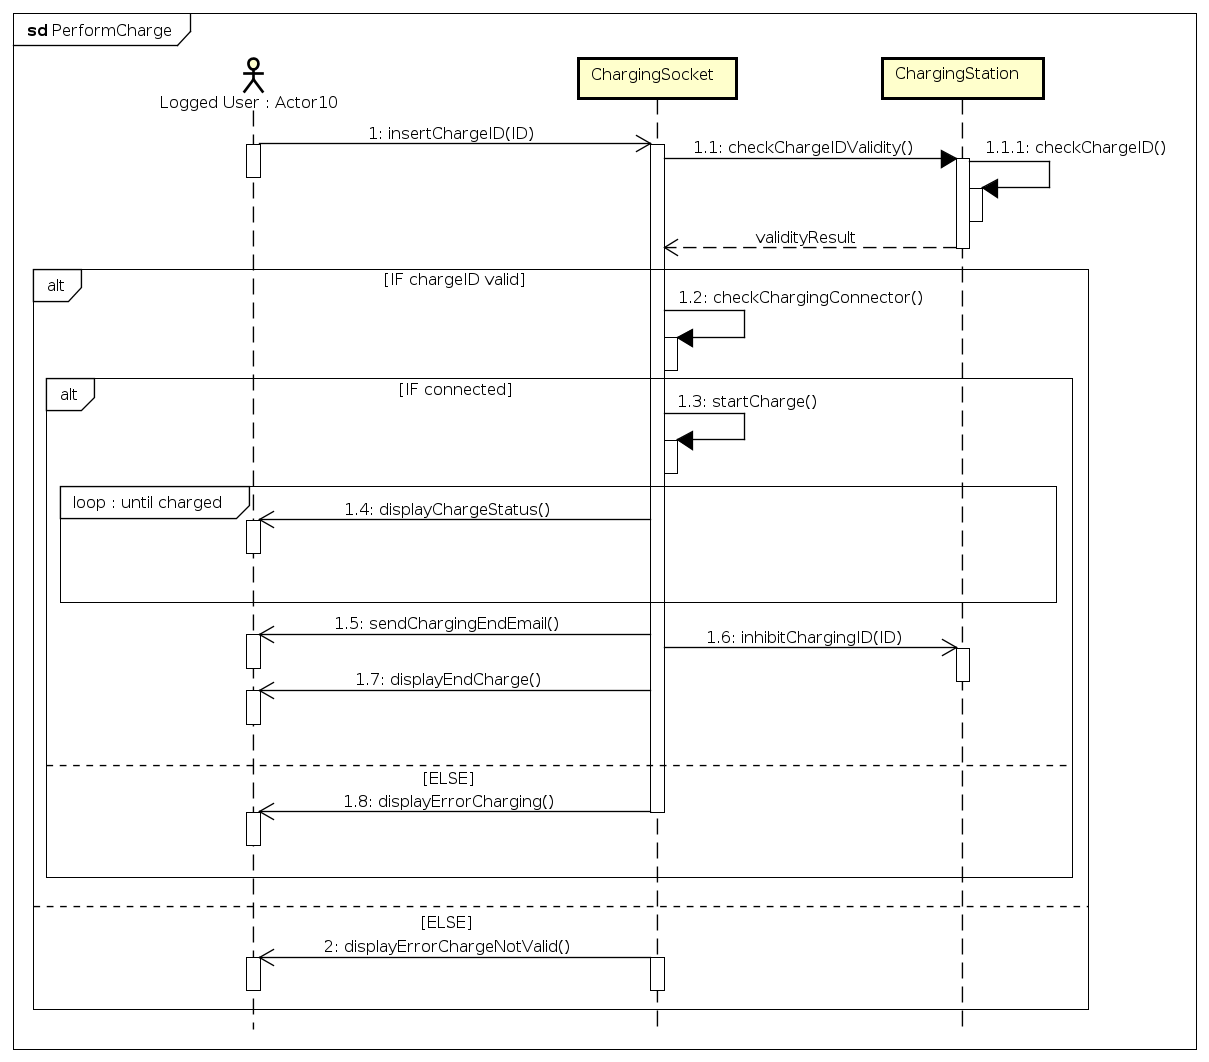
\includegraphics[keepaspectratio, width=16cm]{Sequence/PerformCharge.png}
        \caption{Perform a charge sequence}
    \end{center}
\end{figure}
\begin{figure}[!h]
    \begin{center}
        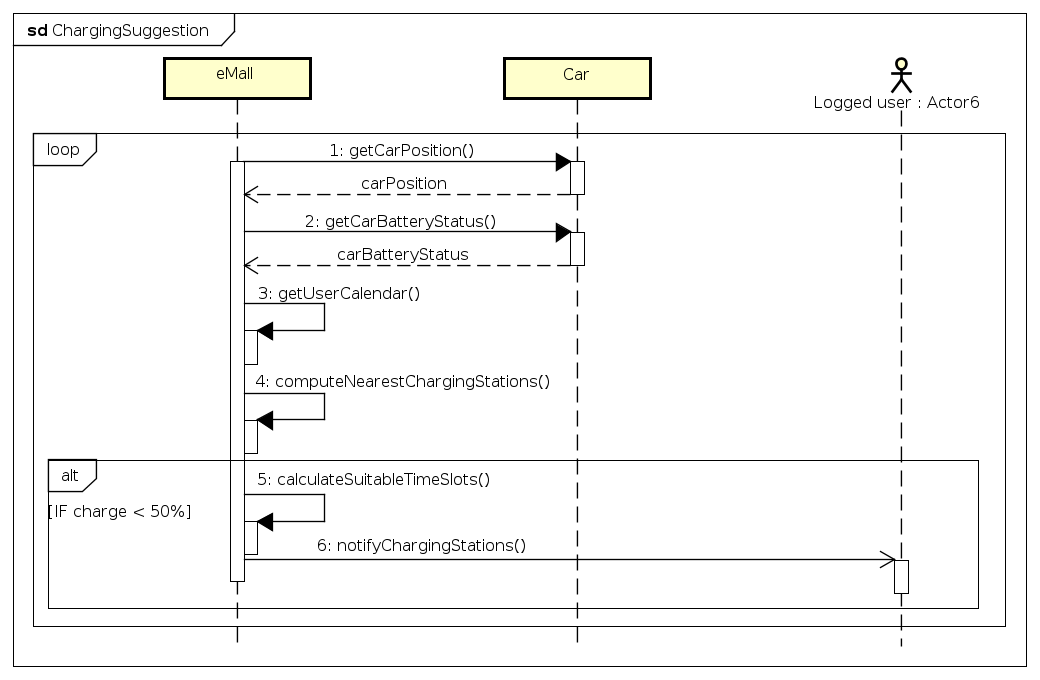
\includegraphics[keepaspectratio, width=16cm]{Sequence/ChargingSuggestion.png}
        \caption{Charging suggestions via calendar sequence}
    \end{center}
\end{figure}

\clearpage
%Definition of use case diagrams, use cases and associated sequence/activity diagrams, and mapping on requirements
\subsection{Performance requirements}
The system in general needs to manage a large collection of electric car users/\acp{CPO} and it needs to supply the heaviest services (like computing the cheapest nearest stations) in a reasonable amount of time.
Because of that the system shall guarantee a baseline load of 1000000 users/\acp{CPO} still with a response time not greater than 5 seconds. To achieve the goal, the system shall be able to decentralize all the computation as possible,
trying to make the client responsible of the heaviest loads.
\subsection{Design constraints}
\subsubsection{Standards compliance}
The system must meet the following standards:
\begin{itemize}
    \item \textbf{\ac{GDPR} law}: The system must be compliant with the current GDPR law about users privacy;
    \item \textbf{Android and iOS}: The system must be compatible with the current versions and reasonably still used previous ones of Android and iOS.
\end{itemize}
\subsubsection{Hardware limitations}
Because the system consists of a smartphone app, the main hardware limitation is the computational capability of a smartphone processor. Hence the
application must be compatible with a low computational capability.
\subsubsection{Other constraints (TODO MAYBE)}

\subsection{Software system attributes}
\subsubsection{Reliability}
About the reliability, the system should prefer a fail safe scenarios, where the actual service can behave slower than expected but still consistent with the results.
To do so the system should be distributed data wise but also performance wise, allowing a scalability factor while being open for maintenance without completely going down.
Some good techniques are \ac{RACS} and \ac{RAPS} which put the reliability very high in the architecture.
\subsubsection{Availability}
Because as stated before a complete period of down would not be great for this type of service, eMall has to prefer the availability over the actual conformity of response time.
Thus the availability should be as high as possible but greater than 99.99\% and must use some techniques to avoid down time during maintenance.
\subsubsection{Security}
Because the system will handle different personal user data, and because one of the standards that it has to follow is the \ac{GDPR} law, it is required a certain level
of security around the system. So an encryption of the user passwords must be adopted and the access to the user's data must be restricted only to the user itself.
It is important that not even the system administrator could access the user's data in respect of the privacy laws.\\
It needs to be highlighted also that according to the \ac{GDPR} laws, the user has the right to revoke the consent about the usage of the data by the platform. This means that
whenever a user decides to delete the account from the system, all the data must about the user must be deleted permanently.
\subsubsection{Maintainability}
As stated in the Reliability and Availability sections, a good pattern for the whole system would be to consider the maintenance as less invasive as possible, using duplicated data and services.
Thus with this idea it would be not complicated to just maintain a single or a restricted amount of nodes per time. This way the user would only experience at worst slowdowns but never actually downtime.
\subsubsection{Portability}
The system should concretize in an APP for the user's smartphone, so it is important to develop the application as cross platform as possible. Doing so eventual updates and modifies won't need any modify to be actually portable from a device to another.
\subsection{Requirements}
\subsubsection{External Interface Requirements}
\clearpage